\section{Anatomy of the failure}
\label{sec:anatomy}

Two families of explanation come to mind for Section~\ref{sec:paradox}, and both
turn out to be wrong. The first is that question-first degrades the model's
perception of the image. The second is that it is a length or budget effect,
since the two layouts sit differently in the context window. We reject the
second immediately: \sti{} and \sit{} contain exactly the same tokens in a
different order, so their prompt lengths are identical to the token
(Table~\ref{tab:cost}). We spend the rest of this section rejecting the first,
and locating what actually breaks.

\subsection{The question does reach the image, and rewrites it}
\label{sec:anatomy-steering}

Putting the question before the image changes the image tokens themselves. We
compare each ordering's layer-18 image-token states against a run whose input is
the image alone, with no system message and no question, and take the mean
per-patch cosine. Under \ist{}, where nothing precedes the image, the patches are
the image-only patches (mean cosine $0.999998$ over $7{,}600$ pairs). Under
\sit{}, where only the system message precedes them, it falls to $0.9110$. Under
\sti{} it falls to $0.8627$, with the most affected patch at $0.6149$, so the
question-specific rewrite is about $1.8\times$ the size of the system message's
own effect.

Causal masking gives a free control here, and it also explains a later result.
Echoing the question \emph{after} the image (\stit{}) cannot alter the image
tokens, and the measurement confirms it to five decimals:
$\cos(\sti{}, \stit{}) = 0.99999$. Whatever \stit{} does for accuracy, it does
without touching perception.

\subsection{What breaks is read-out, and it breaks late}
\label{sec:anatomy-readout}

If perception is intact, the failure has to be downstream of it. We probe the
answer position directly on the $150$ NaturalBench pairs where \sti{} is wrong
and \sit{} is right, tracking how much attention mass the answer position sends
to the question span and to the image span at each of the model's 36 layers.

At layer 23, where answer-to-question attention peaks for both orderings, \sti{}
sends $0.0676$ of its mass to the question while \sit{} sends $0.1479$, a
$2.19\times$ deficit. Attention to the image runs the other way, peaking at
$0.2367$ for \sti{} against $0.0942$ for \sit{}. Averaged over layers 20 to 35,
the ratio of question to image attention is $0.424$ under \sti{} and $1.065$
under \sit{}. Question-first leaves the answer position staring at the image it
has already encoded, and not at the question it is supposed to answer.

The timing matters as much as the size. Tracking $P(\text{correct})$ over the
$\{$Yes, No$\}$ decision at each layer on $300$ pairs, the two orderings are
indistinguishable at chance ($\approx 0.50$) through layer 25. They separate at
layer 26 and never re-cross: by layer 34, \sti{} is at $0.0986$ and \sit{} at
$0.8747$. A failure that only appears in the last quarter of the network is not
an encoding failure. Logit-lens $P(\text{gt})$ at the final layer tells the same
story, $0.1346$ for \sti{} against $0.8485$ for \sit{}.

\begin{figure}[t]
\begin{center}
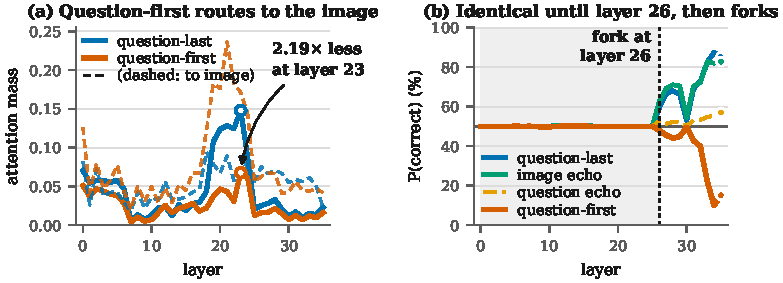
\includegraphics{figs/fig_mechanism.pdf}
\end{center}
\caption{Where question-first breaks (150 NaturalBench pairs where it is wrong
and question-last is right). \textbf{(a)} Attention leaving the answer position,
to the question (solid) and the image (dashed): at layer 23 question-first sends
$2.19\times$ less to the question. \textbf{(b)} $P(\text{correct})$ per layer.
The two baselines sit at chance through layer 25, fork at 26 and never re-cross;
both echo orderings track question-last.}
\label{fig:mechanism}
\end{figure}

\begin{finding}
\textbf{Finding.} The failure is read-out, not perception, and it is late.
Question-first sends $2.19\times$ less attention from the answer position to the
question at the peak read-out layer ($0.0676$ vs $0.1479$), the two orderings
are indistinguishable until layer 26 of 36, and they then diverge to
$P(\text{correct})$ of $0.0986$ versus $0.8747$.
\end{finding}

\subsection{A causal test: severing the two paths dissociates the orderings}
\label{sec:anatomy-knockout}

\begin{wrapfigure}{r}{0.44\textwidth}
\vspace{-14pt}
\begin{center}
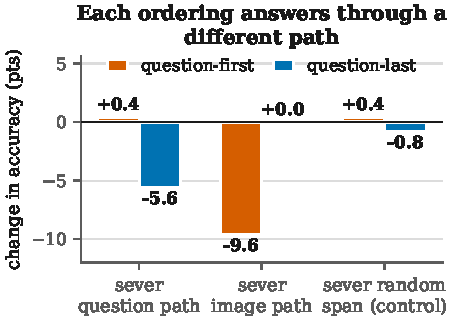
\includegraphics[width=0.42\textwidth]{figs/fig_knockout.pdf}
\end{center}
\vspace{-9pt}
\caption{Attention knockout, 250 NaturalBench pairs, query side restricted to
the answer position. Bars are change against the unmodified run.}
\label{fig:knockout}
\vspace{-10pt}
\end{wrapfigure}
The attention numbers are correlational. To show that the question path is what
\sit{} depends on and the image path is what \sti{} depends on, we sever each
one and measure the damage. We zero the attention edges from the answer position
to the question span (\texttt{ko\_question}) or to the image span
(\texttt{ko\_image}), on $250$ NaturalBench pairs, and add a control that severs
an equal-length random span of pre-image text (\texttt{ko\_random}) so that any
effect of merely removing attention mass is accounted for.

The result is a clean double dissociation (Figure~\ref{fig:knockout}). Cutting
the answer-to-question path costs \sit{} $5.6$ points ($58.8 \to 53.2$, paired
bootstrap 95\% CI $[+1.99, +9.60]$) and costs \sti{} nothing at all ($+0.4$).
Cutting the answer-to-image path costs \sti{} $9.6$ points ($57.6 \to 48.0$) and
costs \sit{} exactly zero. The random-span control moves both orderings by at
most $0.8$ points, so neither effect is an artifact of removing attention mass.

Question-last answers by reading the question. Question-first answers by reading
the image, having already folded its reading of the question into those image
tokens, and that is the path that does not carry the answer.


\begin{finding}
\textbf{Finding.} The two orderings answer through different paths, and we show
it causally. Severing answer-to-question costs \sit{} $5.6$ points (95\% CI
$[+1.99, +9.60]$) and \sti{} nothing ($+0.4$); severing answer-to-image costs
\sti{} $9.6$ points and \sit{} nothing ($0.0$); a span-size control moves both
by $\leq 0.8$.
\end{finding}
